\documentclass{article}

\usepackage{graphicx} % Per immagini
\usepackage{tabularx} % Per creare tabelle styfel
%\setlength\parindent{0pt} % Rimuove indendazioni
\usepackage[utf8x]{inputenc} %serve per i simboli utf8x
\usepackage[italian]{babel}

%\usepackage{subcaption} %serve per mettere le subfigure ESCLUDE SUBFIG

\usepackage{times} % Uncomment to use the Times New Roman font
\usepackage{siunitx}
\usepackage{textgreek}
\usepackage{multirow}
\usepackage{siunitx}
%\usepackage{textcomp}
%\usepackage{fancyhdr}
\usepackage{float} %serve per mettere le immagini in posizione Here
%\usepackage{subfig} %serve per mettere più figure in colonna o in riga
\usepackage[a4paper,total={170mm,257mm},left=25mm,right=25mm,bottom=35mm]{geometry} % per il layout



\begin{document}

\title{DOCUMENTAZIONE PROGETTO INGEGNERIA DEL SOFTWARE}

\author{Cracco Andrea\\Litterini Simone\\Alessio Meneghini }

\date{\today}

\maketitle

\vspace{1.5cm}

\newpage


\section{descrizione del progetto}

sadsa
d
as
d
sa
d


\section{USE CASE del software}

	\vspace{0.5cm}

	\begin{figure}[H]

		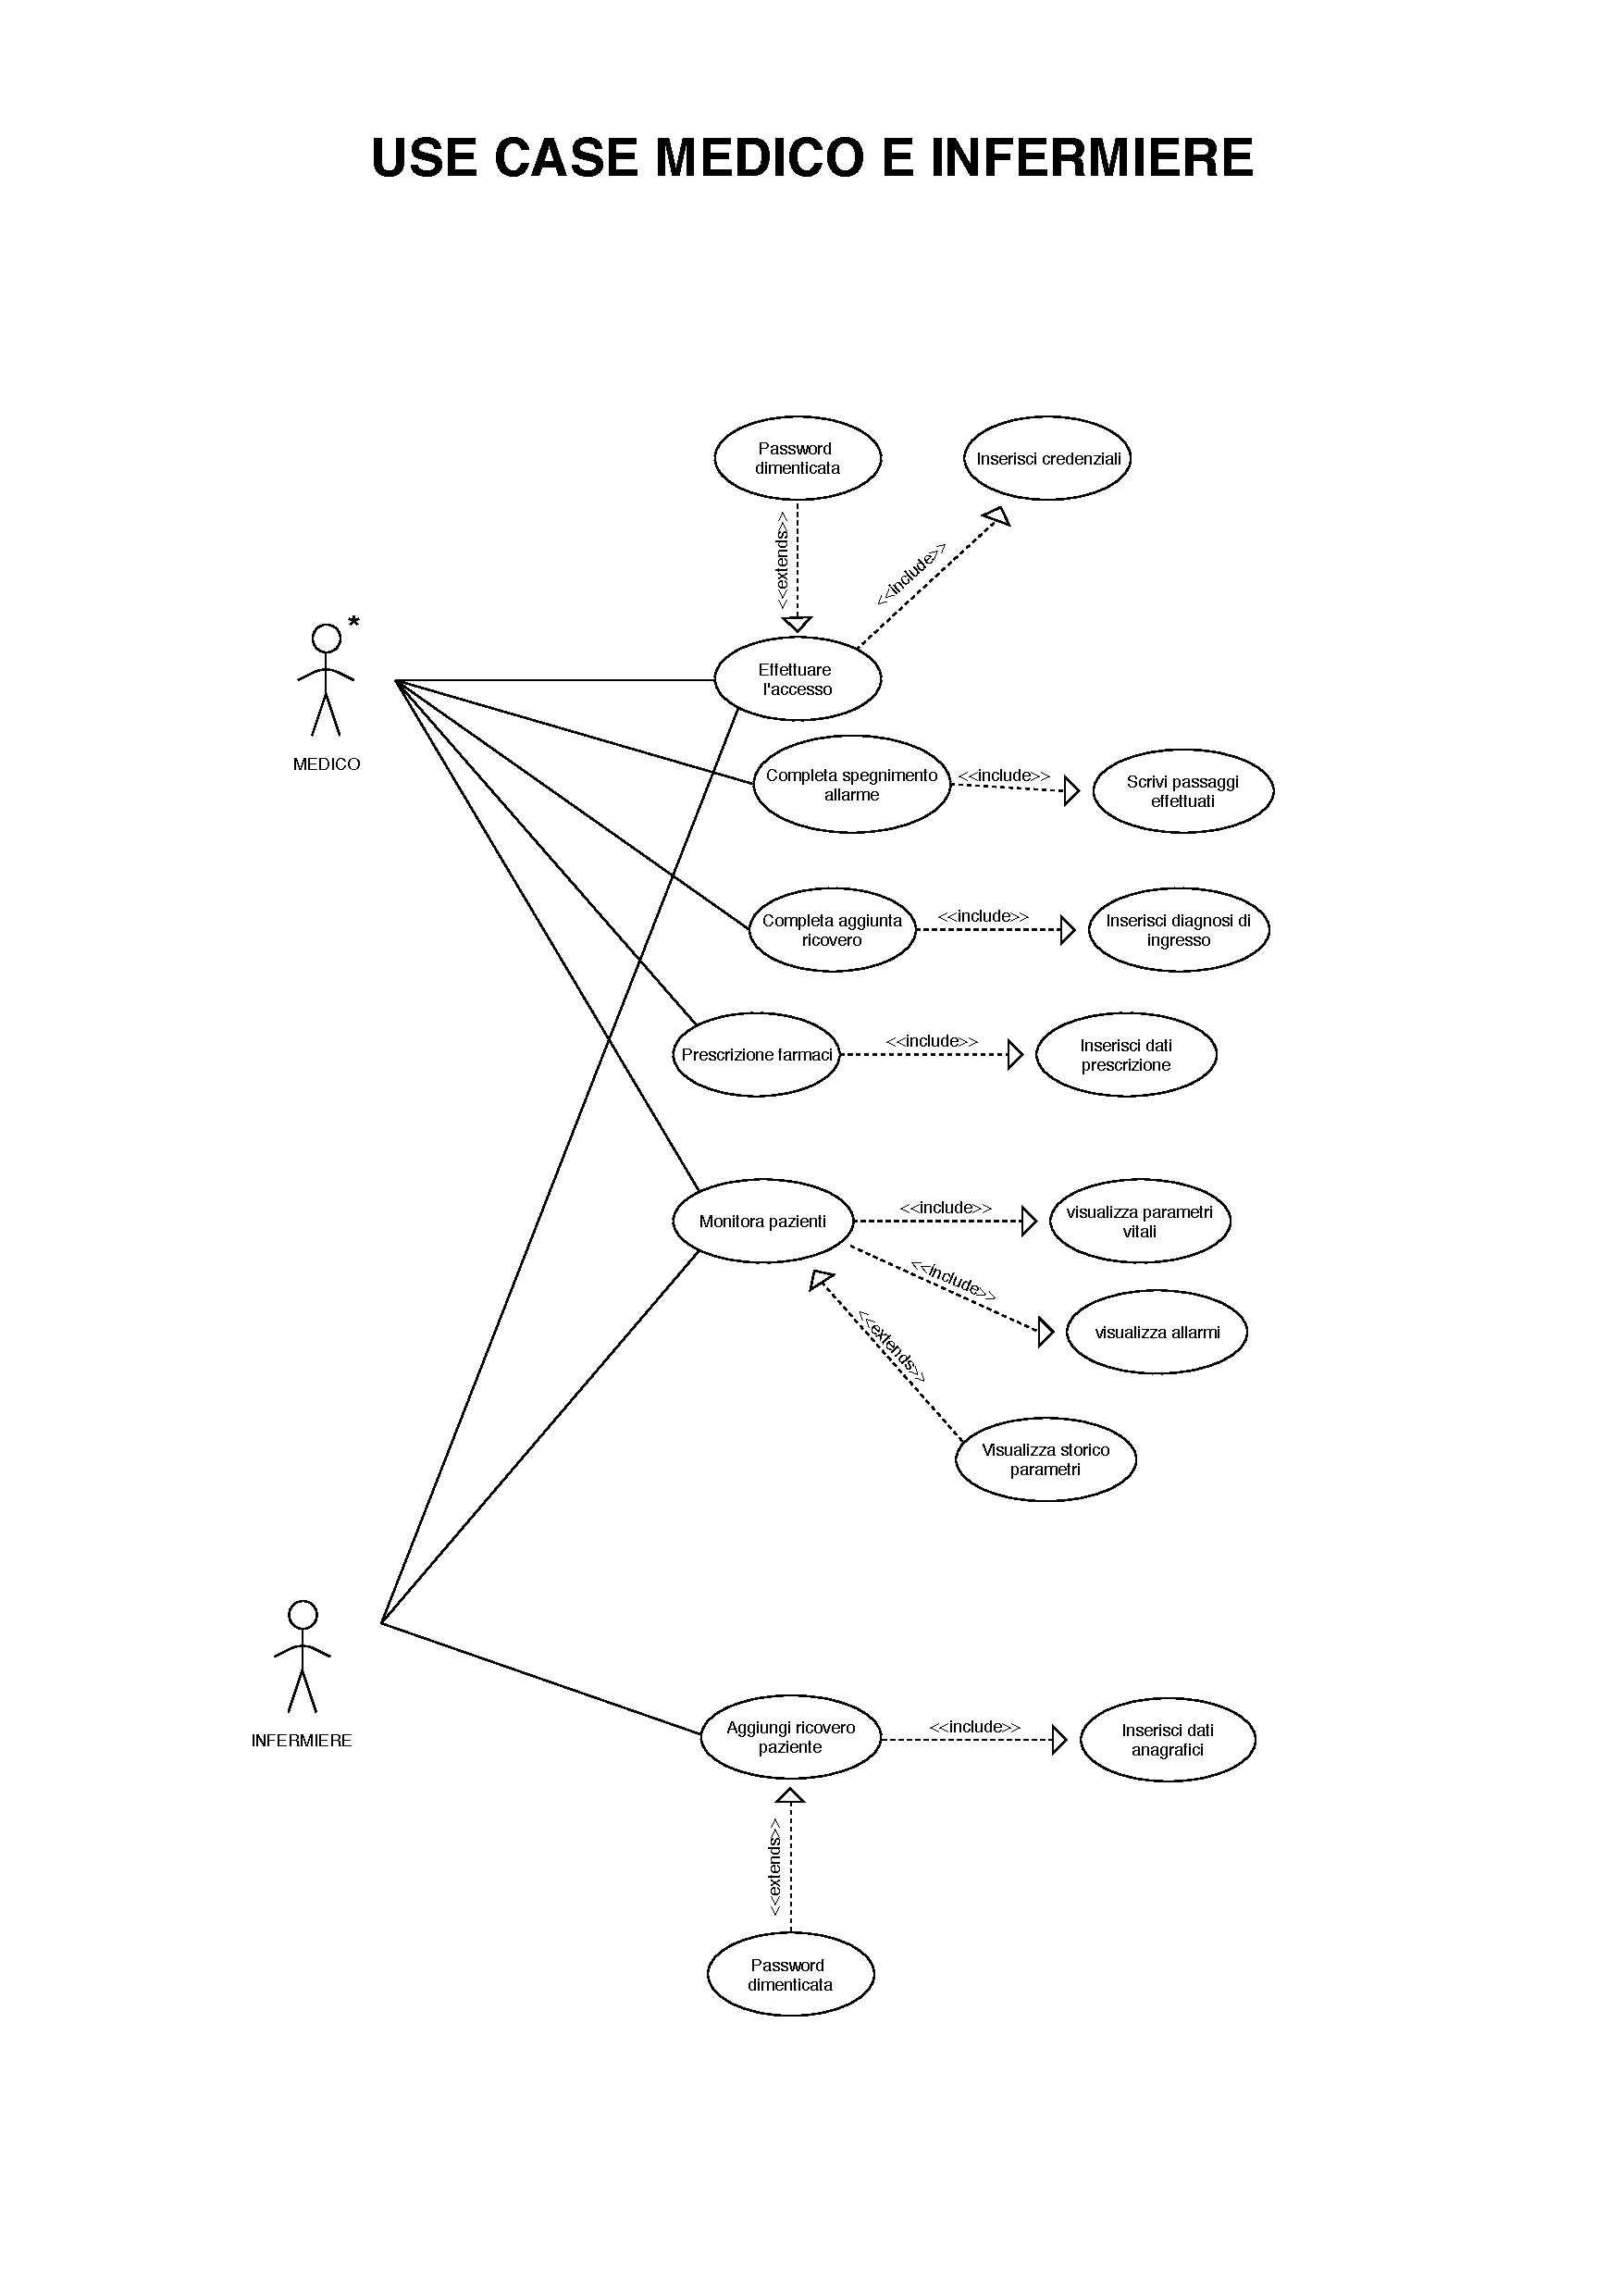
\includegraphics[width=0.9\textwidth]{documenti/useCase_infermiere.pdf}
		\caption{Use case del medico e dell'infermiere con le varie attività che possono svolgere.}
		\label{usecase_medico_infermiere}

	\end{figure}

	\vspace{0.5cm}

	\begin{figure}[H]

		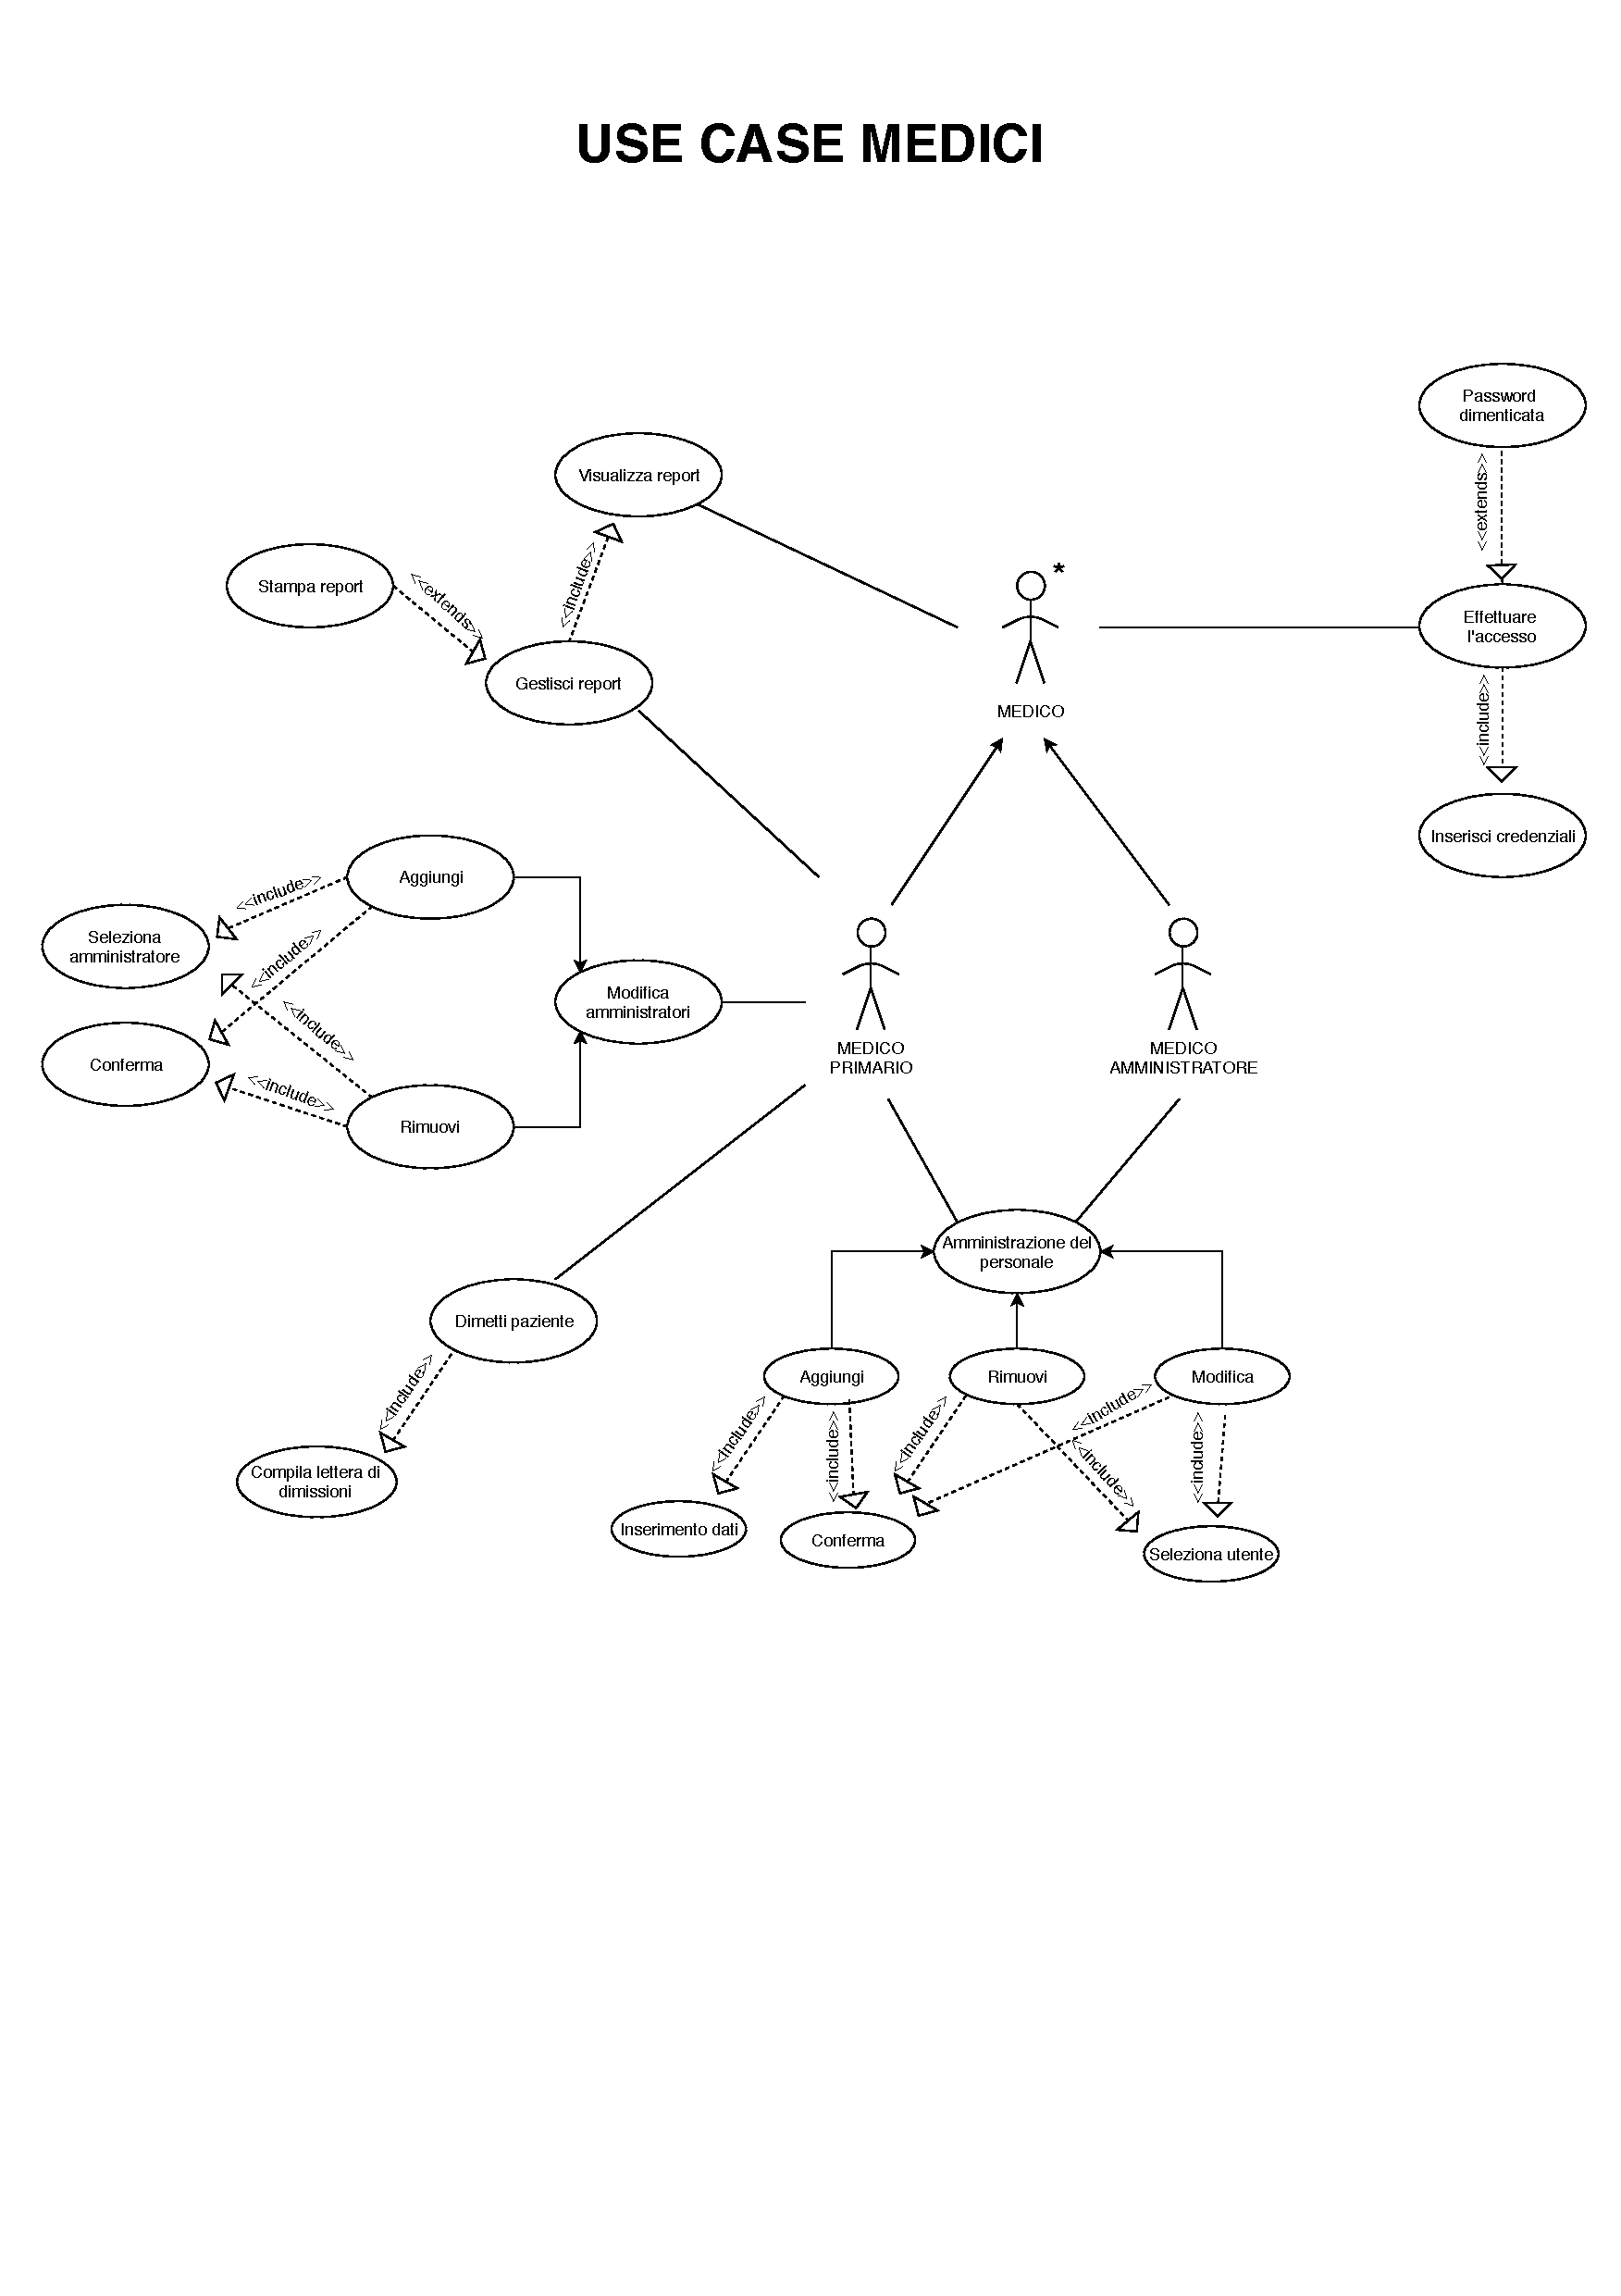
\includegraphics[width=0.9\textwidth]{documenti/useCase_medici.pdf}
		\caption{Use case delle relative sottoclassi di medico, come per esempio ammnistratore o primario.  E le attività che possono svolgere}
		\label{usecase_medici}

	\end{figure}

	\vspace{0.5cm}


\newpage




\section{USE CASE principali con i relativi diagrammi di attività e di sequenza}

\subsection{"Log-in" use case}

Use case per il Log-in. Descrive la procedura da seguire per eseguire l'autenticazioen di un utente per poter poi entrare nella schermata di monitoraggio vera e propria, differente per tipologia di utente. 

\vspace{1cm}

\begin{center}

	\begin{tabular}{r@{\vspace{0.4cm}}ll}
	

	\hline
	
	\textbf{Template UseCase} & \textbf{          "Log-in" use case } \\

	\hline
	
	\multicolumn{1}{c}{Attori}  & Medico e Infermiere \\

	\cline{1-1}
\hline

	\multicolumn{1}{c}{Pre-Condizioni}  & Il server deve essere attivo per potersi collegare alle macchine ed al database.\\ \cline{1-1}&

La connessione deve essere attiva per la trasmissione dei pacchetti di rete con il server, \\&
Inoltre il server e il Database devono essere online ( presume ci sia la connessione sulla macchina ).\\

\hline
	\multicolumn{1}{c}{Sequenza}    \\ \cline{1-1}&
 1. L’utente inserisce l’username \\&
    2. L’utente inserisce la password \\&
    3. preme il pulsante di “Log-in”\\&
    4. Vengono inviate le credenziali al server e si attende  \\&
	    5. Il server crea fa una domanda al database tramite query SQL \\&
    6. Se nel database c’è un istanza in utente che cincide con username e password, l’autenticazione è garantita \\

\hline
	
\multicolumn{1}{c}{Post-Condizioni}  & Il Frame di autenticazione scompare e viene mostrato il monitor con I pazienti \\ \cline{1-1}
\hline

\multicolumn{1}{c}{Sequenza alternativa}  \\     \cline{1-1}&

1. L’utente non si ricorda più la password \\&
     2. Preme il pulsante di “password dimenticata”\\&
        3. L’utente inserisce una mail valida(collegata al proprio account)  \\&
	    4. L’utente conferma tramite il pulsante  \\&
        5. Il server riceve i dati inseriti e controlla la validità della mail \\&
    6. Se la mail è valida, viene inviata una mail con la nuova password all’utente.\\

\hline

	\end{tabular}

\end{center}


\begin{figure}[H]

		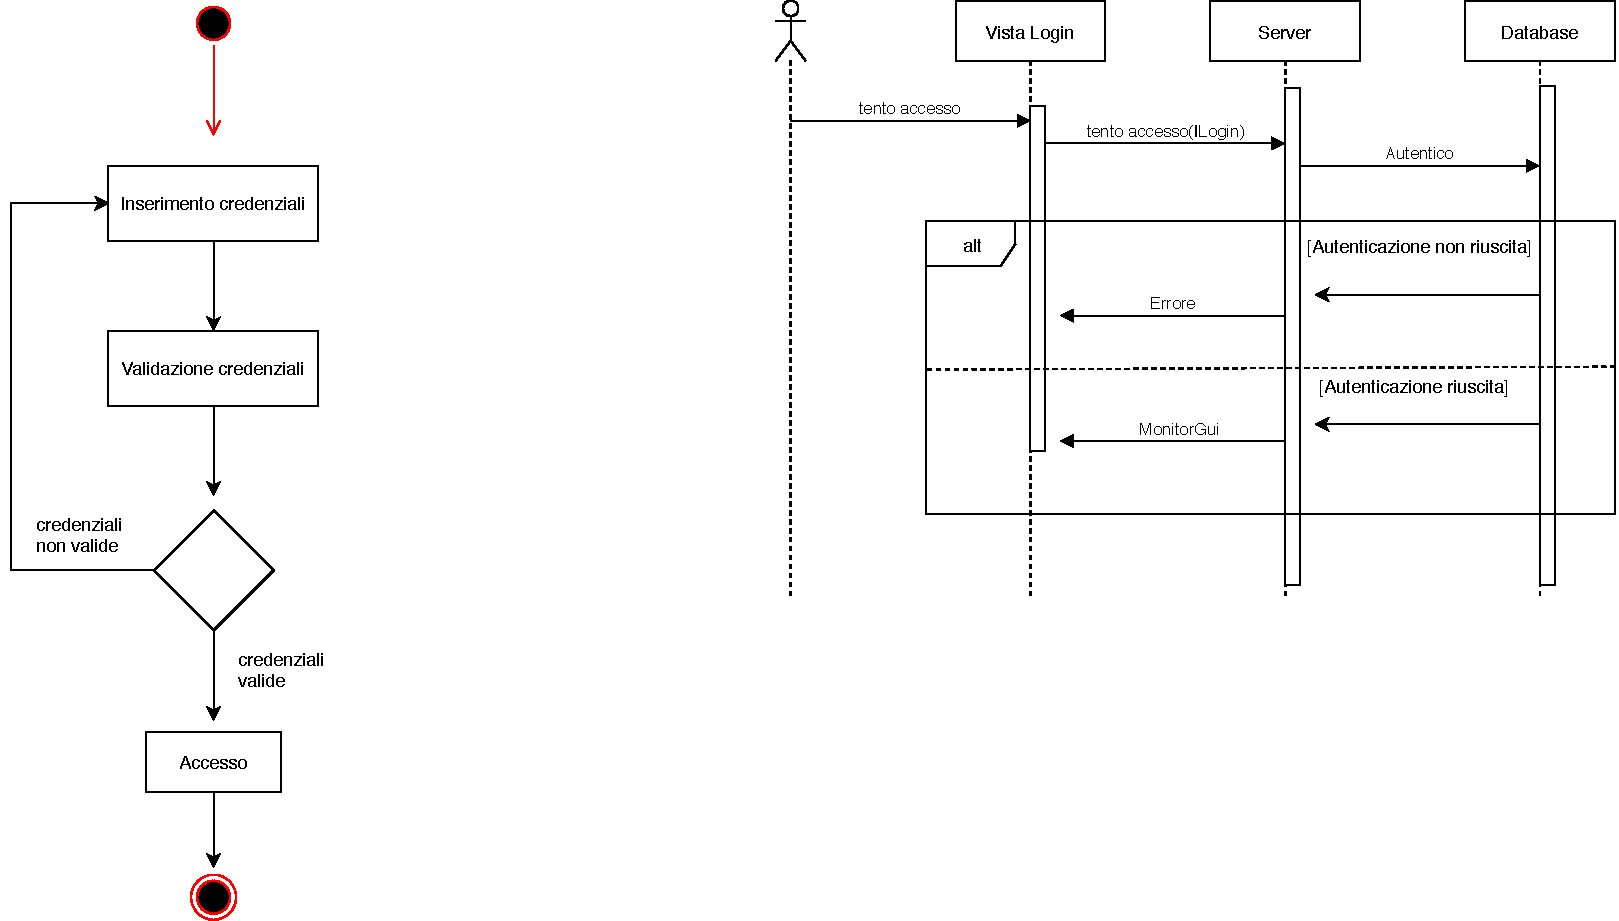
\includegraphics[width=1.1\textwidth]{documenti/Activity_Sequence_diagram_Login.pdf}
		\caption{Activity e sequence diagram del Log-in usecase}
		\label{ActivitySequencediagramLogin}

\end{figure}


\vspace{2cm}




\subsection{"Aggiunta ricovero" use case}

Use case della procedura di aggiunta ricovero, descrive il metodo per aggiungere un nuovo ricovero nel database. Può essere eseguito da infermieri e medici.

\vspace{1cm}

\begin{center}

	\begin{tabular}{r@{\vspace{0.4cm}}ll}
	

	\hline
	
	\textbf{Template UseCase  } &  \textbf{       "Aggiunta ricovero" use case } \\

	\hline
	
	\multicolumn{1}{c}{Attori}  & Infermiere o Medico(in caso non ci siano infermieri) \\

	\cline{1-1}
\hline

	\multicolumn{1}{c}{Pre-Condizioni}  & L’utente deve aver fatto l’autenticazione e deve essere\\ \cline{1-1}&

un utente di tipo infermiere o medico, Inoltre il server e il Database devono essere online\\&
( presume ci sia la connessione sulla macchina ).\\

\hline
	\multicolumn{1}{c}{Sequenza}    \\ \cline{1-1}&
    1. L’utente preme il pulsante verde sul monitor \\&
    2. L’utente deve inserire tutti I dati pertinenti all’aggunta di un nuovo ricovero \\&
    3. Preme il pulsante di aggiunta nuovo ricovero\\&
    4. Il server riceve I dati pertinenti al nuovo paziente da ricoverare  \\&
    5.Il server tramite una query al database in SQL aggiunge se non esiste già il nuovo ricovero  \\

\hline
	
\multicolumn{1}{c}{Post-Condizioni}  &Al monitor dei pazienti viene aggiunto un nuovo PatientMonitor \\ \cline{1-1}&

che mostra Il paziente con I relativi dati e parametri vitali\\
\hline

\multicolumn{1}{c}{Sequenza alternativa}  \\     


\hline

	\end{tabular}

\end{center}

\vspace{2cm}


\begin{figure}[H]

		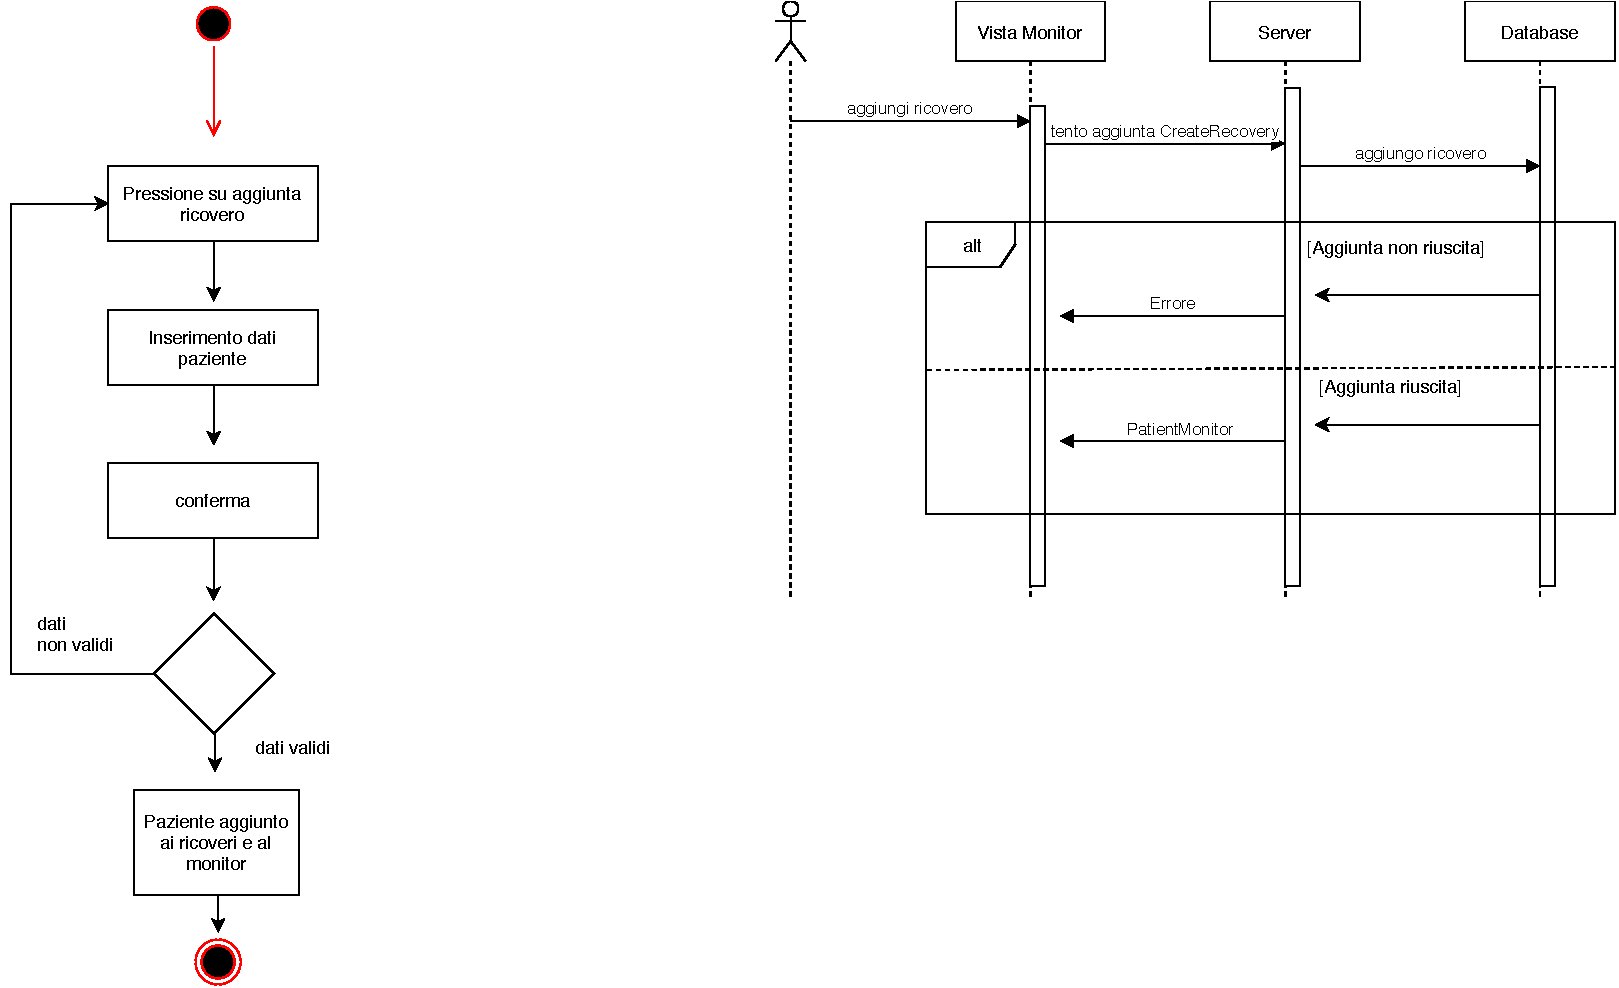
\includegraphics[width=1.1\textwidth]{documenti/Activity_Sequence_diagram_Ricovero.pdf}
		\caption{Activity e sequence diagram del Log-in usecase}
		\label{Activity_Sequence_diagram_Login}

	\end{figure}


\vspace{2cm}



\subsection{"Gestione utenti" use case}

Use case per la gestione degli utenti, permette ad un amministratore di aggiungere, rimuovere o modificare un utente medico o infermiere nel database degli utenti.

\vspace{1cm}

\begin{center}

	\begin{tabular}{r@{\vspace{0.4cm}}ll}
	

	\hline
	
	\textbf{Template UseCase} & \textbf{          "Gestione utenti" use case } \\

	\hline
	
	\multicolumn{1}{c}{Attori}  & Medico amministratore o primario
 \\

	\cline{1-1}
\hline

	\multicolumn{1}{c}{Pre-Condizioni}  & Essere loggato come amministratore o primario.\\&
il server e il Database devono essere online ( presume ci sia la connessione sulla macchina ).\\

\hline
	\multicolumn{1}{c}{Sequenza}    \\ \cline{1-1}&
 1. Il medico primario o amministratore inserisce i dati dell’utente da aggiungere \\&
    2.    Il medico primario o amministratore preme il pulsante aggiungi; \\&
    3. Il server riceve i dati del nuovo utente\\&
    4. Il server, tramite una query SQL, aggiunge l’utente al database se non è già presente. \\
   
\hline
	
\multicolumn{1}{c}{Post-Condizioni}  &Il nuovo utente è stato aggiunto al database utenti\\ \cline{1-1}
\hline

\multicolumn{1}{c}{Sequenza alternativa (rimozione)}  \\     \cline{1-1}&

1.Il medico primario o amministratore seleziona l’utente da rimuovere \\&
         2. Il medico preme il pulsante di conferma;\\&
            3. Il server con una query SQL rimuove l’utente selezionato dal database.\\
\hline

\multicolumn{1}{c}{Sequenza alternativa (modifica)}  \\     \cline{1-1}&

1. Il medico seleziona l’utente da modificare \\&
     2. l medico inserisce i dati che vuole modificare al posto di quelli presenti\\&
        3. Il server con una query SQL modifica le informazioni relative all’utente se\\& i nuovi dati sono corretti e compatibili  \\&
	    4. L’utente conferma tramite il pulsante  \\

\hline

	\end{tabular}

\end{center}


\begin{figure}[H]

		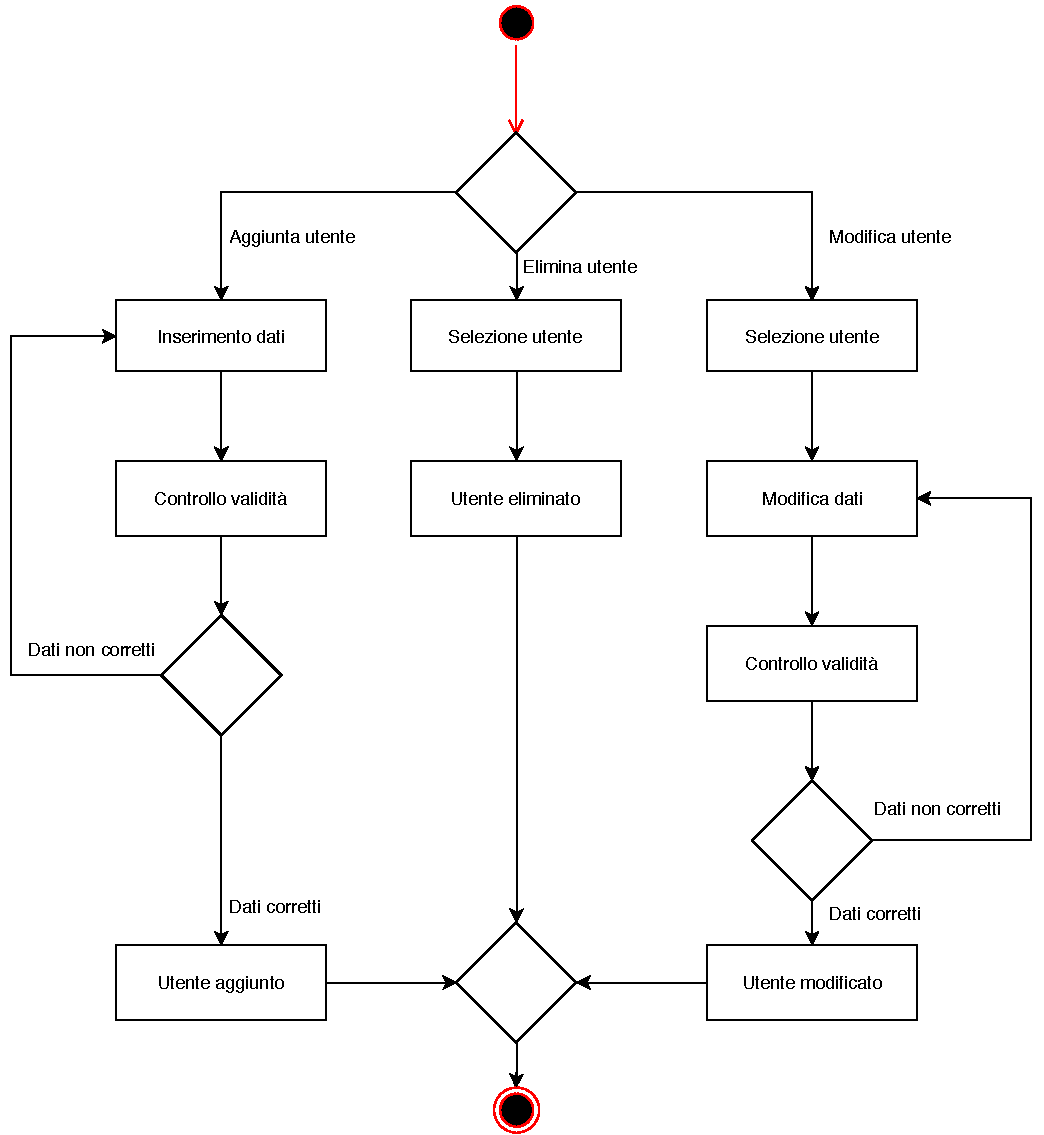
\includegraphics[width=1.1\textwidth]{documenti/Activity_diagram_getioneUtenti.pdf}
		\caption{Activity diagram "gestione utenti" use case}
		\label{sequence_diagram_getioneUtenti}

	\end{figure}

\vspace{2cm}

\begin{figure}[H]

		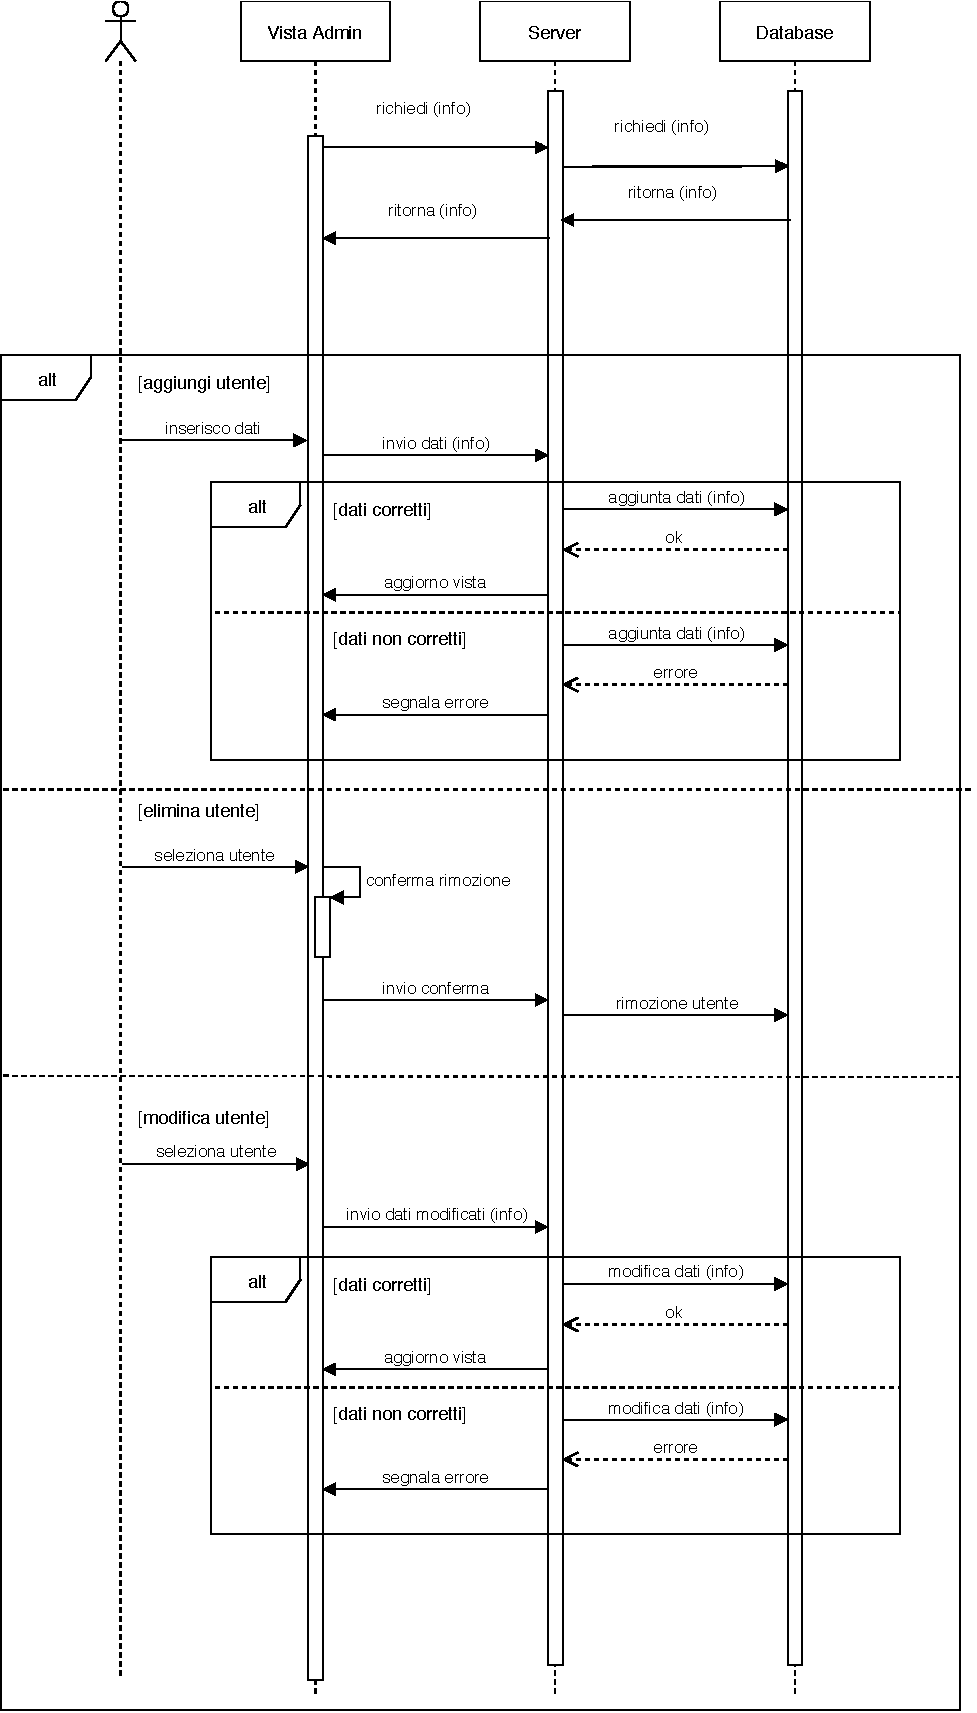
\includegraphics[width=0.9\textwidth]{documenti/sequence_diagram_getioneUtenti.pdf}
		\caption{Sequence diagram "gestione utenti" use case}
		\label{Activity_diagram_getioneUtenti}

	\end{figure}



\vspace{2cm}


\subsection{"Prescription" use case}

Use case per la prescrizione farmaci, consente di aggiungere prescrizioni di farmaci ai pazienti nel database nel caso in cui ci si sia loggati come medici e il sistema verifica i privilegi.

\vspace{1cm}

\begin{center}

	\begin{tabular}{r@{\vspace{0.4cm}}ll}
	

	\hline
	
	\textbf{Template UseCase  } &  \textbf{       "Prescription" use case } \\

	\hline
	
	\multicolumn{1}{c}{Attori}  & Medico \\

	\cline{1-1}
\hline

	\multicolumn{1}{c}{Pre-Condizioni}  & L’utente deve aver fatto l’autenticazione e deve essere\\ \cline{1-1}&

un utente di tipo Medico , inoltre server e Database devono essere online ( presume macchina connessa )\\

\hline
	\multicolumn{1}{c}{Sequenza}    \\ \cline{1-1}&
    1.  Il medico clicca cerca farmaco; \\&
    2. Il database dei farmaci ritorna la lista di farmaci \\&
    3. Il medico aggiunge i dati del paziente e invia\\&
    4. Il server invia con una query SQL la prescrizione  \\&
    5.Il database la registra  \\

\hline
	
\multicolumn{1}{c}{Post-Condizioni}  &La prescrizione è registrata sul database correttamente \\ \cline{1-1}
\hline

\multicolumn{1}{c}{Sequenza alternativa}  \\     

\hline

	\end{tabular}

\end{center}




\begin{figure}[H]

		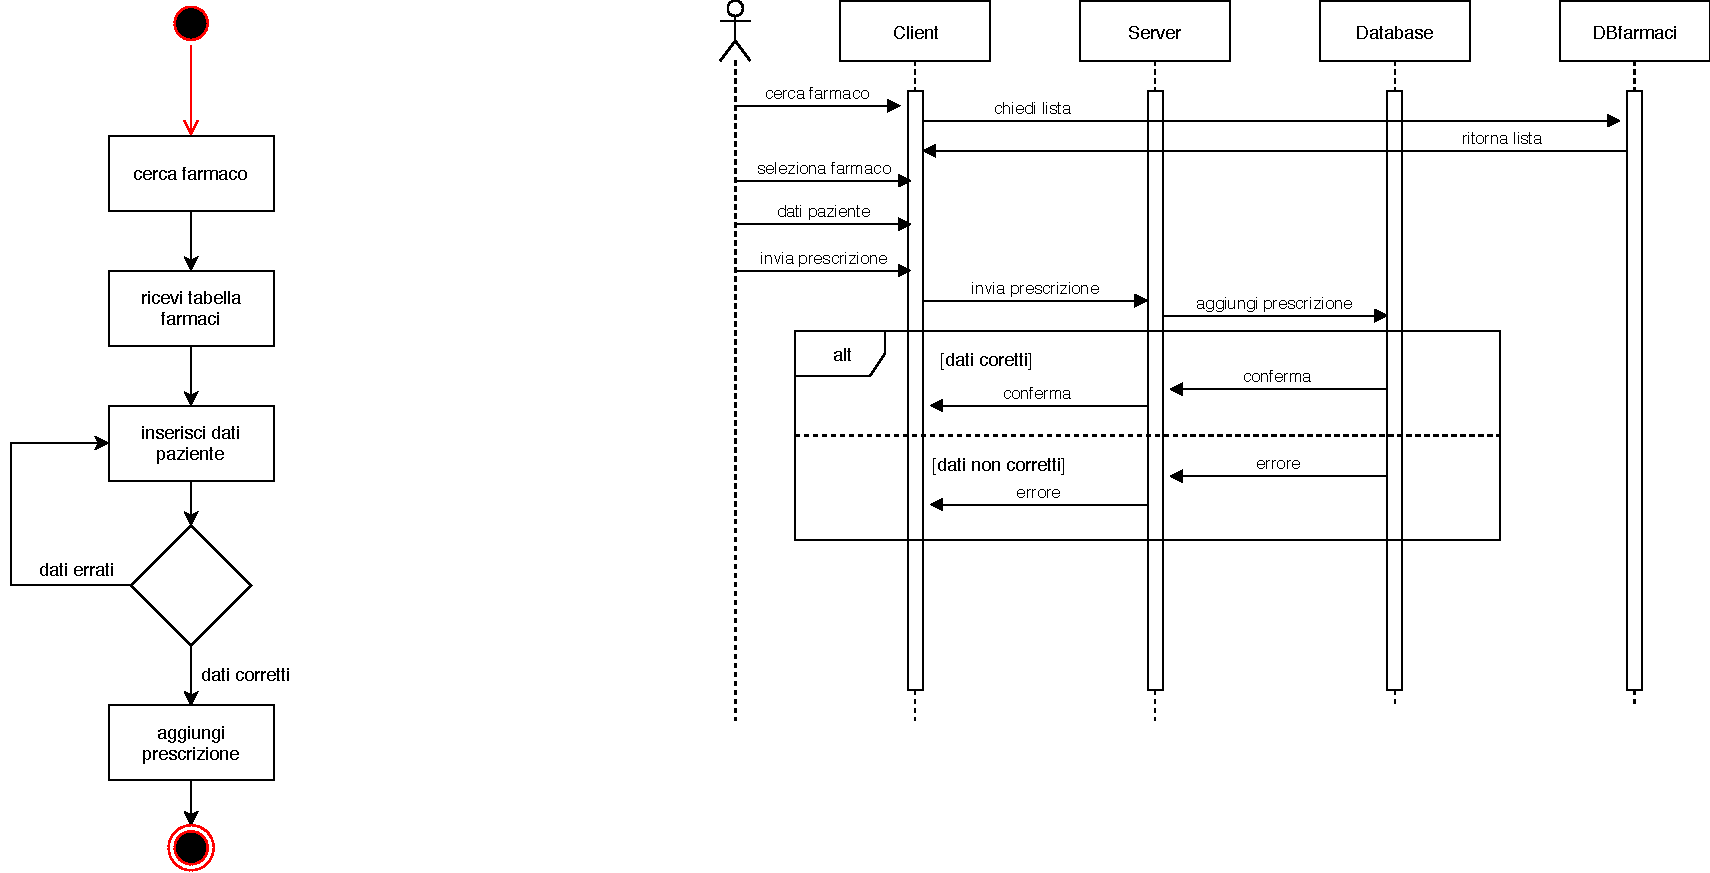
\includegraphics[width=1.1\textwidth]{documenti/Diagrams_prescrizioni.pdf}
		\caption{Activity e sequence diagram del "Prescription" usecase}
		\label{Diagrams_prescrizioni}

	\end{figure}


\vspace{2cm}


\subsection{"Alarm monitor" use case}

Use case per la gestione dei dati dei monitor e dei relativi allarmi, gestisce l’aggiornamento sincronizzato dei monitor con server e client, attiva l’allarme se i valori sono fuori da quelli accettabili, spegne l’allarme quando i valori tornano nei range di tolleranza.

\vspace{1cm}

\begin{center}

	\begin{tabular}{r@{\vspace{0.4cm}}ll}
	

	\hline
	
	\textbf{Template UseCase  } &  \textbf{       "Alarm monitor" use case } \\

	\hline
	
	\multicolumn{1}{c}{Attori}  & Monitor, Server, Client \\

	\cline{1-1}
\hline

	\multicolumn{1}{c}{Pre-Condizioni}  & Monitor e server accesi e connessi\\ 


\hline
	\multicolumn{1}{c}{Sequenza (aggiornamento) }    \\ \cline{1-1}&
    1.  Il monitor aggiorna i propri dati \\&
    2. Il monitor invia i dati aggiornati al server \\&
    3. Il server invia i dati ricevuti ai client connessi in quel momento\\&
    4.Il client si aggiorna con i dati ricevuti dal server  \\
    

\hline
	
\multicolumn{1}{c}{Post-Condizioni}  &Le informazioni visualizzate sul client sono le stesse fornite dal monitor \\ \cline{1-1}
\hline

\multicolumn{1}{c}{Sequenza alternativa (allarme)}     \\ \cline{1-1}&

 1.  Il monitor aggiorna i propri dati \\&
    2.Il monitor rileva valori anormali e invia l’allarme al server \\&
    3. Il server passa l’allarme e i valori al client\\&
    4. Il client aggiorna i dati e segnala l’allarme con il simbolo di pericolo e un suono  \\

\hline

	\end{tabular}

\end{center}




\begin{figure}[H]

		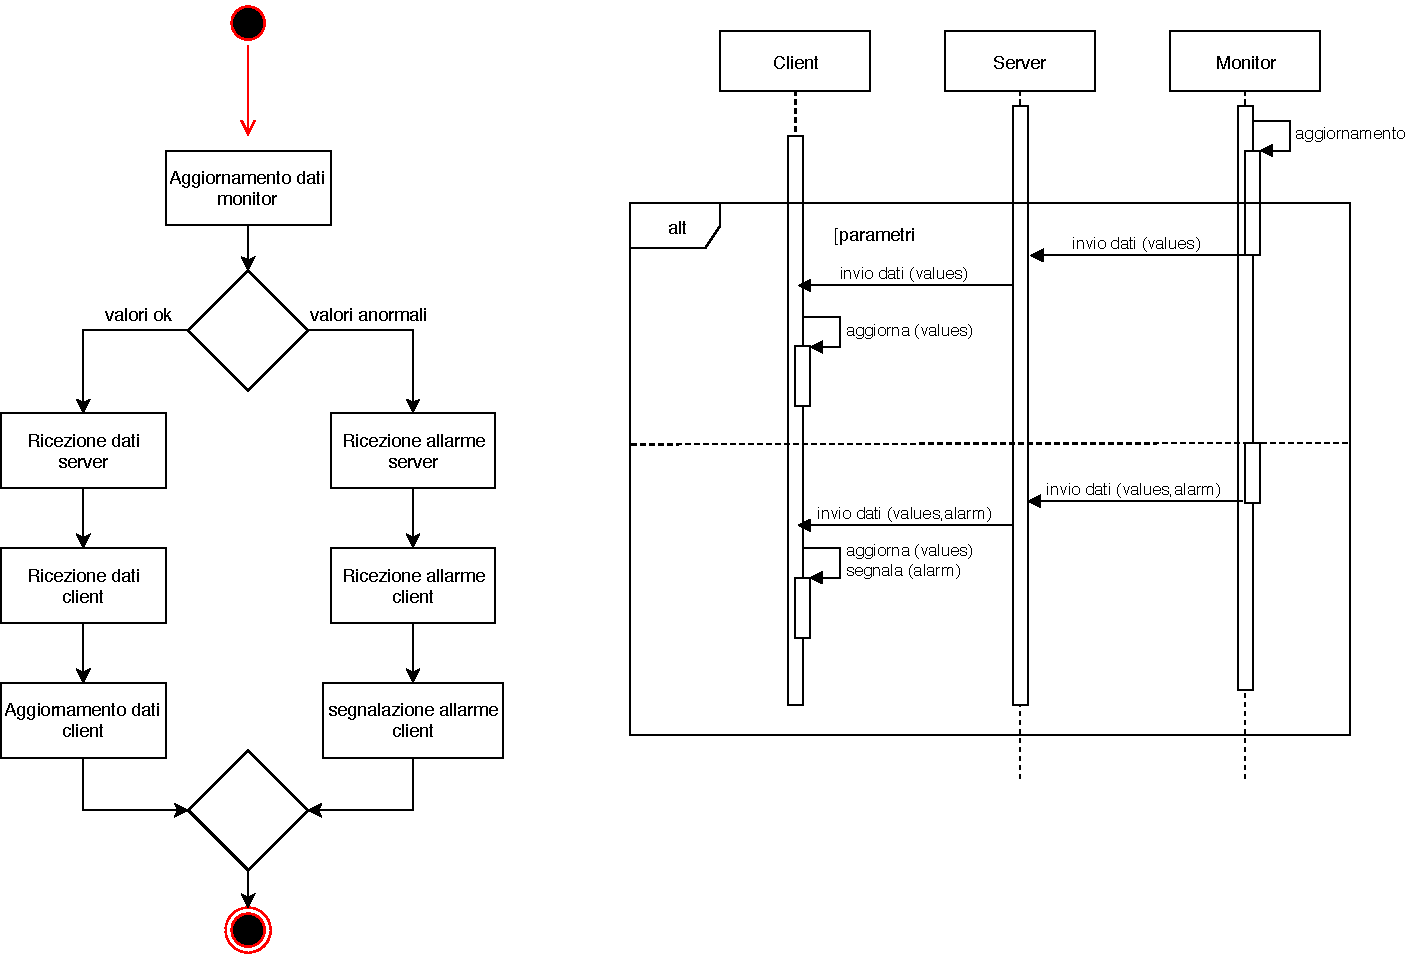
\includegraphics[width=1.1\textwidth]{documenti/Diagrams_monitorAgg.pdf}
		\caption{Activity e sequence diagram del "Alarm monitor" usecase}
		\label{Diagrams_monitorAgg}

	\end{figure}


\vspace{2cm}
















\end{document}